% Template for PLoS
% Version 3.5 March 2018
%
% % % % % % % % % % % % % % % % % % % % % %
%
% -- IMPORTANT NOTE
%
% This template contains comments intended
% to minimize problems and delays during our production
% process. Please follow the template instructions
% whenever possible.
%
% % % % % % % % % % % % % % % % % % % % % % %
%
% Once your paper is accepted for publication,
% PLEASE REMOVE ALL TRACKED CHANGES in this file
% and leave only the final text of your manuscript.
% PLOS recommends the use of latexdiff to track changes during review, as this will help to maintain a clean tex file.
% Visit https://www.ctan.org/pkg/latexdiff?lang=en for info or contact us at latex@plos.org.
%
%
% There are no restrictions on package use within the LaTeX files except that
% no packages listed in the template may be deleted.
%
% Please do not include colors or graphics in the text.
%
% The manuscript LaTeX source should be contained within a single file (do not use \input, \externaldocument, or similar commands).
%
% % % % % % % % % % % % % % % % % % % % % % %
%
% -- FIGURES AND TABLES
%
% Please include tables/figure captions directly after the paragraph where they are first cited in the text.
%
% DO NOT INCLUDE GRAPHICS IN YOUR MANUSCRIPT
% - Figures should be uploaded separately from your manuscript file.
% - Figures generated using LaTeX should be extracted and removed from the PDF before submission.
% - Figures containing multiple panels/subfigures must be combined into one image file before submission.
% For figure citations, please use "Fig" instead of "Figure".
% See http://journals.plos.org/plosone/s/figures for PLOS figure guidelines.
%
% Tables should be cell-based and may not contain:
% - spacing/line breaks within cells to alter layout or alignment
% - do not nest tabular environments (no tabular environments within tabular environments)
% - no graphics or colored text (cell background color/shading OK)
% See http://journals.plos.org/plosone/s/tables for table guidelines.
%
% For tables that exceed the width of the text column, use the adjustwidth environment as illustrated in the example table in text below.
%
% % % % % % % % % % % % % % % % % % % % % % % %
%
% -- EQUATIONS, MATH SYMBOLS, SUBSCRIPTS, AND SUPERSCRIPTS
%
% IMPORTANT
% Below are a few tips to help format your equations and other special characters according to our specifications. For more tips to help reduce the possibility of formatting errors during conversion, please see our LaTeX guidelines at http://journals.plos.org/plosone/s/latex
%
% For inline equations, please be sure to include all portions of an equation in the math environment.  For example, x$^2$ is incorrect; this should be formatted as $x^2$ (or $\mathrm{x}^2$ if the romanized font is desired).
%
% Do not include text that is not math in the math environment. For example, CO2 should be written as CO\textsubscript{2} instead of CO$_2$.
%
% Please add line breaks to long display equations when possible in order to fit size of the column.
%
% For inline equations, please do not include punctuation (commas, etc) within the math environment unless this is part of the equation.
%
% When adding superscript or subscripts outside of brackets/braces, please group using {}.  For example, change "[U(D,E,\gamma)]^2" to "{[U(D,E,\gamma)]}^2".
%
% Do not use \cal for caligraphic font.  Instead, use \mathcal{}
%
% % % % % % % % % % % % % % % % % % % % % % % %
%
% Please contact latex@plos.org with any questions.
%
% % % % % % % % % % % % % % % % % % % % % % % %

\documentclass[10pt,letterpaper]{article}
\usepackage[top=0.85in,left=2.75in,footskip=0.75in]{geometry}

% amsmath and amssymb packages, useful for mathematical formulas and symbols
\usepackage{amsmath,amssymb}

% Use adjustwidth environment to exceed column width (see example table in text)
\usepackage{changepage}

% Use Unicode characters when possible
\usepackage[utf8x]{inputenc}

% textcomp package and marvosym package for additional characters
\usepackage{textcomp,marvosym}

% cite package, to clean up citations in the main text. Do not remove.
\usepackage{cite}

% Use nameref to cite supporting information files (see Supporting Information section for more info)
\usepackage{nameref,hyperref}

% line numbers
\usepackage[right]{lineno}

% ligatures disabled
\usepackage{microtype}
\DisableLigatures[f]{encoding = *, family = * }

% color can be used to apply background shading to table cells only
\usepackage[table]{xcolor}

% array package and thick rules for tables
\usepackage{array}

% create "+" rule type for thick vertical lines
\newcolumntype{+}{!{\vrule width 2pt}}

% create \thickcline for thick horizontal lines of variable length
\newlength\savedwidth
\newcommand\thickcline[1]{%
  \noalign{\global\savedwidth\arrayrulewidth\global\arrayrulewidth 2pt}%
  \cline{#1}%
  \noalign{\vskip\arrayrulewidth}%
  \noalign{\global\arrayrulewidth\savedwidth}%
}

% \thickhline command for thick horizontal lines that span the table
\newcommand\thickhline{\noalign{\global\savedwidth\arrayrulewidth\global\arrayrulewidth 2pt}%
\hline
\noalign{\global\arrayrulewidth\savedwidth}}


% Remove comment for double spacing
%\usepackage{setspace}
%\doublespacing

% Text layout
%\raggedright
\setlength{\parindent}{0.5cm}
\textwidth 5.25in
\textheight 8.75in

% Bold the 'Figure #' in the caption and separate it from the title/caption with a period
% Captions will be left justified
\usepackage[aboveskip=1pt,labelfont=bf,labelsep=period,justification=raggedright,singlelinecheck=off]{caption}
\renewcommand{\figurename}{Fig}

% Use the PLoS provided BiBTeX style
\bibliographystyle{plos2015}

% Remove brackets from numbering in List of References
\makeatletter
\renewcommand{\@biblabel}[1]{\quad#1.}
\makeatother



% Header and Footer with logo
\usepackage{lastpage,fancyhdr,graphicx}
\usepackage{epstopdf}
%\pagestyle{myheadings}
\pagestyle{fancy}
\fancyhf{}
%\setlength{\headheight}{27.023pt}
%\lhead{\includegraphics[width=2.0in]{PLOS-submission.eps}}
\rfoot{\thepage/\pageref{LastPage}}
\renewcommand{\headrulewidth}{0pt}
\renewcommand{\footrule}{\hrule height 2pt \vspace{2mm}}
\fancyheadoffset[L]{2.25in}
\fancyfootoffset[L]{2.25in}
\lfoot{\today}

\usepackage{mathtools}
%% Include all macros below

%% END MACROS SECTION

\begin{document}
\vspace*{0.2in}

% Title must be 250 characters or less.
\begin{flushleft}
{\Large
\textbf\newline{OpenSim Moco: Musculoskeletal optimal control} % Please use "sentence case" for title and headings (capitalize only the first word in a title (or heading), the first word in a subtitle (or subheading), and any proper nouns).
}
\newline
% Insert author names, affiliations and corresponding author email (do not include titles, positions, or degrees).
\\
Christopher L. Dembia\textsuperscript{1\Yinyang*},
Nicholas A. Bianco\textsuperscript{1\Yinyang},
Antoine Falisse\textsuperscript{2},
Jennifer L. Hicks\textsuperscript{3},
Scott L. Delp\textsuperscript{1,3,4}
\\
\bigskip
\textbf{1} Department of Mechanical Engineering, Stanford University, Stanford, California, United States of America
\\
\textbf{2} Department of Movement Sciences, KU Leuven, Leuven, Belgium
\\
\textbf{3} Department of Bioengineering, Stanford University, Stanford, California, United States of America
\\
\textbf{4} Department of Orthopaedic Surgery, Stanford University, Stanford, California, United States of America
\\
\bigskip

% Insert additional author notes using the symbols described below. Insert symbol callouts after author names as necessary.
%
% Remove or comment out the author notes below if they aren't used.
%
% Primary Equal Contribution Note
\Yinyang These authors contributed equally to this work.

% Additional Equal Contribution Note
% Also use this double-dagger symbol for special authorship notes, such as senior authorship.
%\ddag These authors also contributed equally to this work.

% Current address notes
%\textcurrency Current Address: Dept/Program/Center, Institution Name, City, State, Country % change symbol to "\textcurrency a" if more than one current address note
% \textcurrency b Insert second current address
% \textcurrency c Insert third current address

% Deceased author note
%\dag Deceased

% Group/Consortium Author Note
%\textpilcrow Membership list can be found in the Acknowledgments section.

% Use the asterisk to denote corresponding authorship and provide email address in note below.
* dembia@alumni.stanford.edu

\end{flushleft}
% Please keep the abstract below 300 words
\section*{Abstract}
Musculoskeletal simulations are used in many different applications, ranging from the design of wearable robots that interact with humans to the analysis of patients with impaired movement. Here, we introduce OpenSim Moco, a software toolkit for optimizing the motion and control of musculoskeletal models built in the OpenSim modeling and simulation package. OpenSim Moco uses the direct collocation method, which is often faster and can handle more diverse problems than other methods for musculoskeletal simulation. Moco frees researchers from implementing direct collocation themselves---which typically requires extensive technical expertise---and allows them to focus on their scientific questions. The software can handle a wide range of problems that interest biomechanists, including motion tracking, motion prediction, parameter optimization, model fitting, electromyography-driven simulation, and device design. Moco is the first musculoskeletal direct collocation tool to handle kinematic constraints, which are common in musculoskeletal models. To show Moco's abilities, we first solved for muscle activity that produced an observed walking motion while minimizing muscle excitations and knee joint loading. Next, we predicted how muscle weakness may cause deviations from a healthy walking motion. Lastly, we predicted a squat-to-stand motion and optimized the stiffness of an assistive device placed at the knee. We designed Moco to be easy to use, customizable, and extensible, thereby accelerating the use of simulations to understand human and animal movement.


% Please keep the Author Summary between 150 and 200 words
% Use first person. PLOS ONE authors please skip this step.
% Author Summary not valid for PLOS ONE submissions.
% \section*{Author summary}

\linenumbers

% Use "Eq" instead of "Equation" for equation citations.
\section*{Introduction}

Musculoskeletal simulations have shed light on movement disorders by, for example, discovering ways to walk that reduce knee loading~\cite{Fregly:2007ac}, revealing that children with cerebral palsy exhibit simplified motor control when walking~\cite{Steele:2015}, and reproducing eye disorders that cause double vision~\cite{Priamikov:2016}. Beyond human health and performance, researchers use musculoskeletal simulations to understand how animals move, for example by studying dinosaur locomotion~\cite{sthaya:2005uk} and differences between human and chimpanzee strength~\cite{ONeill:2017}.

Simulations of movement are often categorized by whether the motion is prescribed from experimental data or predicted by the simulation. One may prescribe the motion of a musculoskeletal model to match a motion measured in an experiment~\cite{Thelen:2003bba,Lloyd:2003} to estimate unmeasured quantities such as muscle-level energy consumption~\cite{Farris:2014du,Jackson:2017go}. Existing prescribed motion methods are rapid but are not customizable (e.g., cost functions are predefined) or lack support for important model features such as muscle dynamics.
Motion prediction~\cite{Geijtenbeek:2019} can establish cause-effect relationships (e.g., discovering gait impairments that arise from weakness or contracture~\cite{Ong:2019}) and help design clinical interventions (e.g., prostheses~\cite{Handford:2016kd}).
However, methods for predicting motions often require waiting many hours or days for a solution, so researchers often simplify the model's musculature or reduce the dimensionality of the control scheme.
A third category, which lies between prescribing and predicting motion, is tracking motion, where errors between model kinematics and reference data are part of the cost function rather than exactly prescribed~\cite{Lin:2017jp}.
To accelerate the application of simulations to scientific and clinical questions, researchers need unified simulation tools for solving diverse problems that span the prescribed-to-predicted spectrum and involve a variety of costs and unknown model parameters.

Most musculoskeletal simulations are naturally posed as optimal control problems~\cite{Todorov:2003}. Optimal control problems seek a system's parameters and time-varying controls that minimize a cost (e.g., energy consumption) subject to the system's dynamics, expressed as differential-algebraic equations. An increasingly popular method for solving optimal control problems is to approximate the system's states and controls as polynomial splines and solve for the knot points that lead the spline to obey the system's dynamics~\cite{Betts:2010, Kelly:2017}. The dynamics are enforced by requiring the time derivative of the state splines to match the derivative from the system's differential equations at specified time points. This method is called ``direct collocation'' because the spline derivatives are ``collocated'' with the exact derivatives (\cite{Hairer:1993}, page 211;~\cite{Hairer:1996}, page 498). Direct collocation produces a nonlinear program in which the system states are introduced as variables and the system's dynamics are enforced as constraints. Typical musculoskeletal models lead to optimization problems with thousands of variables. These large problems are tractable with direct collocation because the constraints enforcing the system's dynamics at a given time depend only on the variables near that time.

The advantages of direct collocation have led biomechanists to use the method for prescribing motions~\cite{Groote:2016dq,Ueno:2020}, tracking motions~\cite{Kaplan:2001,Lin:2017jp,Mehrabi:2019}, predicting motions~\cite{Ackermann:2010dd,Ackermann:2012,Miller:2015fc,Porsa:2015dn,Meyer:2016gl,Koelewijn:2016bm,Lee:2016dn,Umberger:2018ec,Bobbert:2016,KMoore:2018ea,Lin:2018ex,Lai:2018,Nguyen:2019,Falisse:2019b,Jansen:2020}, fitting muscle properties~\cite{Falisse:2017}, and optimizing model parameters~\cite{Rohani:2017}. Researchers have made key methodological advances, including efficiently handling multibody and muscle dynamics via implicit formulations~\cite{vandenBogert:2011fv,Groote:2016dq}, minimizing energy consumption~\cite{Koelewijn:2018kw,Koelewijn:2019}, and employing algorithmic differentiation to simulate complex models more rapidly compared to using finite differences~\cite{Falisse:2019a}.

Despite direct collocation's advantages, very few biomechanics laboratories have been able to apply this powerful technique. The method requires arduous bookkeeping of variables and efficient calculation of the objective and constraint function derivatives required by gradient-based optimization algorithms. Several direct collocation solvers exist (e.g.,~\cite{Becerra:2010,Patterson:2014}), but current solvers require users to incorporate their musculoskeletal models manually. OpenSim is a software package used by thousands of biomechanics researchers to model musculoskeletal systems~\cite{Delp:2007ij,Seth:2018gg,Sherman:2011byc}, but OpenSim does not currently employ direct collocation. Several biomechanists have graciously shared their code combining OpenSim or hand-coded models with direct collocation solvers, but such code is tailored to specific models or motions, handles only unconstrained models, or contains closed-source components. Lastly, choosing the problem formulation (e.g., expressing dynamics as explicit or implicit differential equations) and solver settings (e.g., detecting sparsity patterns automatically) that lead to fast convergence requires expertise; ideally, such expertise is embedded into the software via defaults, and users can edit their formulation or solver settings with simple commands.

To improve the accessibility of advanced optimal control methods in musculoskeletal biomechanics, we introduce OpenSim Moco (``musculoskeletal optimal control''), an easy-to-use, customizable, and extensible software toolkit for solving optimal control problems with OpenSim musculoskeletal models (Fig~\ref{overviewmoco}). OpenSim frees biomechanists from implementing equations of motion on their own, and Moco frees biomechanists from implementing direct collocation. Moco not only removes the need to set up gradient-based optimization, but also provides an interface that abstracts away the details of constructing an optimal control problem. With just a few lines of code, researchers can solve complex problems with an OpenSim model for almost any movement. Users can add custom cost terms or constraints if Moco does not provide what they need. This paper details Moco's design and implementation and shows three applications. First, we estimated muscle activity for an observed walking motion and predicted changes in muscle activity with a different cost function. Second, we used Moco to predict how muscle weakness may cause deviations from a healthy walking motion. Finally, to illustrate that Moco can predict motions and model parameters, we predicted a squat-to-stand motion and optimized the stiffness of a passive assistive device.

% Place figure captions after the first paragraph in which they are cited.
\begin{figure}[!h]
%\begin{adjustwidth}{-2.25in}{0in} % Comment out/remove adjustwidth environment if table fits in text column.
    \centering
    % 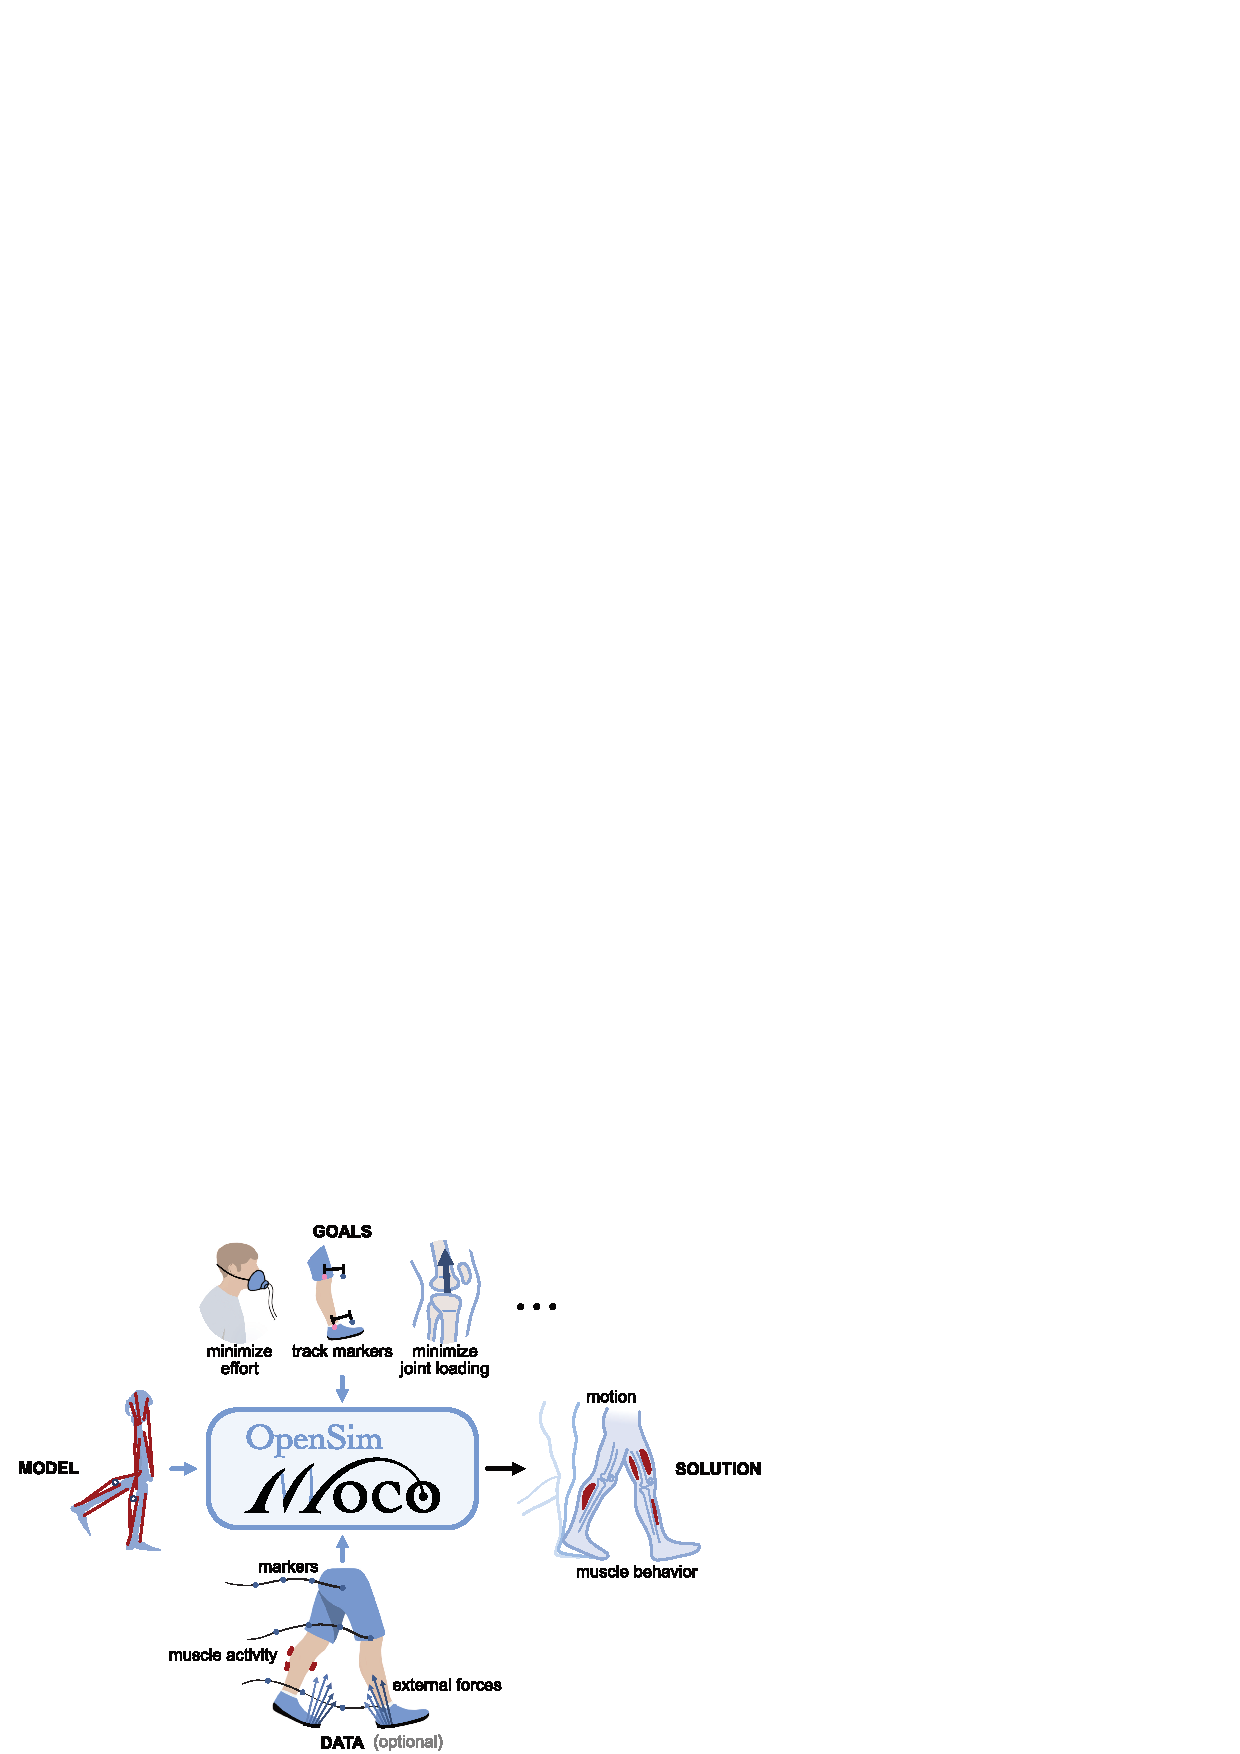
\includegraphics{../figures/OverviewOfMoco.png}
    \caption{{\bf Overview of Moco.}
        OpenSim Moco produces the optimal motion and muscle behavior for a human or animal, given goals to achieve during the motion, an OpenSim musculoskeletal model~\cite{Seth:2018gg}, and reference data. Moco provides a library of goals, such as minimizing effort (illustrated with an indirect calorimetry mask), deviation from marker data (or generalized coordinate data), and joint loading. Reference data for the motion (markers or generalized coordinates), external forces (from force places), and muscle activity (from electromyography) are optional. Illustration credit: Kai Rasmussen.}
    \label{overviewmoco}
%\end{adjustwidth}
\end{figure}

\section*{Design and implementation}

Moco solves optimal control problems that users define using a library of cost and constraint modules, which are implemented through configurable software classes. Users describe their problem with the \textit{MocoProblem} class. (We denote names of classes in Moco and Moco's dependencies with italics.) To decouple the problem from the numerical methods used to solve it, we use the \textit{MocoSolver} class. Moco classes are available via C++, MATLAB, Python, and XML text files, with interfaces familiar to OpenSim users. We package the \textit{MocoProblem} and \textit{MocoSolver} together into a \textit{MocoStudy} (Fig~\ref{mocodiagram}), which can be written to and loaded from XML text files. Moco contains utilities for visualizing and plotting a study's solution, which is held by the \textit{MocoSolution} class. For certain standard biomechanics problems, Moco provides simpler interfaces that may be preferable to the flexibility of \textit{MocoStudy}.

% Place figure captions after the first paragraph in which they are cited.
\begin{figure}[!h]
%\begin{adjustwidth}{-2.25in}{0in} % Comment out/remove adjustwidth environment if table fits in text column.
\centering
    % 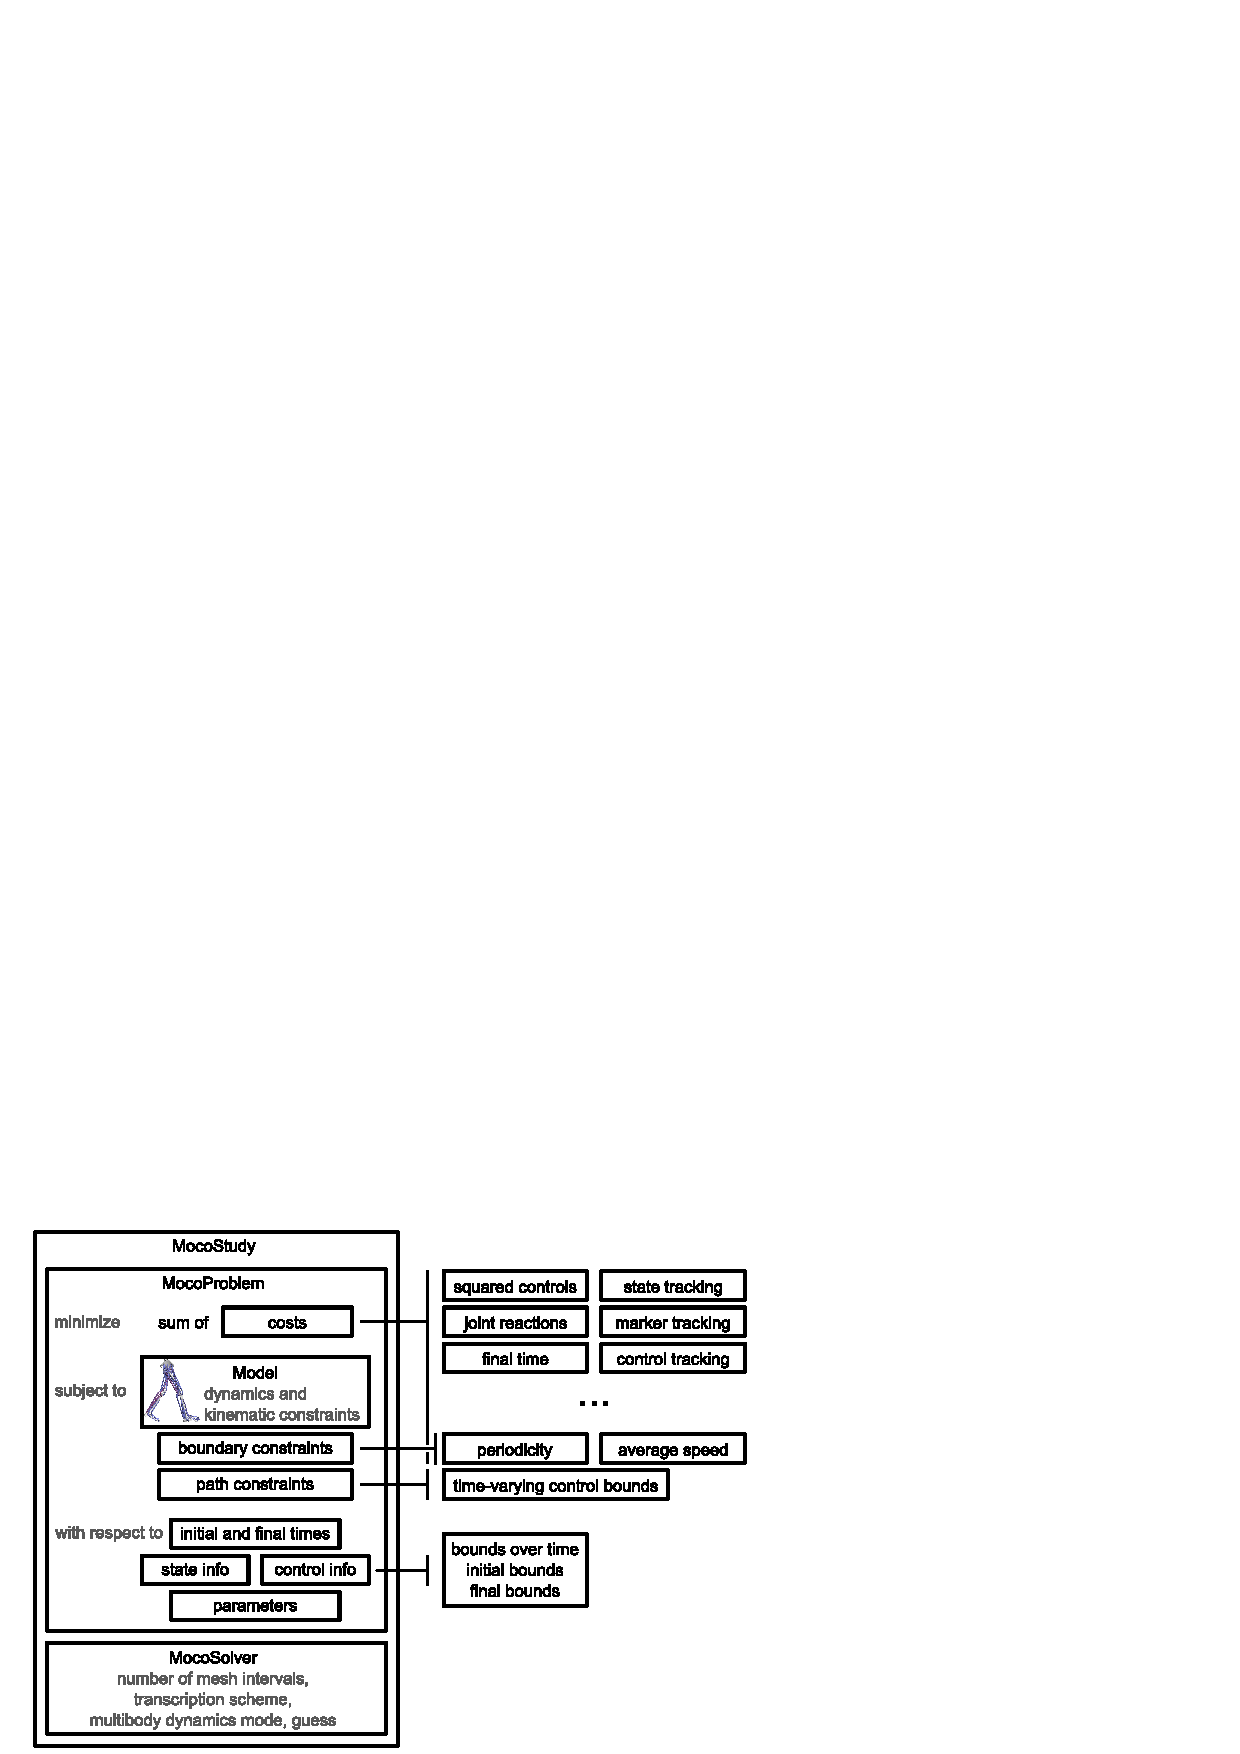
\includegraphics{../figures/MocoStudyDiagram.png}
    \caption{{\bf Overview of \textit{MocoStudy}.}
        Moco solves custom optimal control problems using a library of cost, boundary constraint, and path constraint modules. Moco contains additional cost modules beyond what is shown here, and users can define their own custom modules.}
    \label{mocodiagram}
%\end{adjustwidth}
\end{figure}

\subsection*{Defining problems with \textit{MocoProblem}}

\textit{MocoProblem} supports a diversity of scientific questions and contains the following elements.
\begin{itemize}
\item \textbf{cost terms}: Users can minimize a weighted sum of control effort, deviation from an observed motion, joint reaction loads, the duration of a motion, and other costs by appending to the \textit{MocoProblem} an instance of the class associated with a cost module (e.g., \textit{MocoControlGoal} implements the control effort cost).
\item \textbf{multibody dynamics, muscle dynamics, and kinematic constraints}:
OpenSim \textit{Models} are a standard way to describe musculoskeletal systems, and Moco uses OpenSim \textit{Models} to obtain the system's multibody dynamics, auxiliary dynamics (e.g., muscle activation dynamics and tendon compliance), and kinematic constraints. Moco handles kinematic constraints (using a method by Posa and colleagues~\cite{Posa:2016}), which are commonly used to model anatomy such as the knee, shoulder, and neck~\cite{Seth:2016,Lerner:2015,Rajagopal:2016ek,Cazzola:2017}.
\item \textbf{boundary constraints}: Users can enforce average speed, symmetry, or periodicity with constraints relating initial and final states.
\item \textbf{path constraints}: Users can constrain any function of time to lie in a specified range over the motion. For example, researchers often estimate muscle activity with electromyography and Moco allows constraining simulated muscle excitations to be close to those measurements via the \textit{MocoControlBoundConstraint} class.
\item \textbf{parameter optimization}: Users can optimize model properties, such as a body's mass, a muscle's optimal fiber length, or an exoskeleton's stiffness.
\item \textbf{bounds on variables}: Users can bound the values of states, controls, and initial and final time.
\end{itemize}
For a detailed mathematical description of the problems supported by Moco, consult S1 Appendix.

The modules of a \textit{MocoProblem} can be combined in diverse ways. The following examples illustrate the breadth of problems that users can solve.
\begin{itemize}
\item \textbf{dynamically-constrained inverse kinematics}: Minimize the error between experimental and model marker positions (marker tracking) and control effort while obeying multibody dynamics.
\item \textbf{electromyography-constrained muscle force estimation}: For a prescribed experimental motion, minimize muscle excitations while obeying multibody dynamics and constraining the difference between muscle excitations and electromyography data.
\item \textbf{torso mass calibration}: For a prescribed experimental motion, minimize residual forces at the pelvis while obeying multibody dynamics.
\item \textbf{prediction of muscle coordination adaptations to an exoskeleton}: Minimize squared muscle excitations and the error between experimental joint angles and model coordinate values (state tracking) while obeying multibody and muscle dynamics.
\end{itemize}

We demonstrate Moco's interface in Fig~\ref{mocoexamplecode} with a simple MATLAB example. Setting the model and adding a cost (termed ``goal'' in the code) each require only a single statement.

% Place figure captions after the first paragraph in which they are cited.
\begin{figure}[!h]
    %\begin{adjustwidth}{-2.25in}{0in} % Comment out/remove adjustwidth environment if table fits in text column.
    \centering
    % \includegraphics{../figures/MocoExampleCode.png}
    \caption{{\bf Example code for a simple problem.}
        This MATLAB code uses Moco to find the force to apply to a point mass to move the mass by one meter (starting and ending at rest) in minimum time. Solving this problem requires only 9 lines of code.}
    \label{mocoexamplecode}
    %\end{adjustwidth}
\end{figure}

Direct collocation relies on gradient-based optimization, which converges faster and more reliably when all functions in the problem are continuous and differentiable. Moco includes a continuous and differentiable muscle model \textit{DeGrooteFregly2016Muscle}~\cite{Groote:2016dq}. We extended this muscle model to include damping, which further improves convergence but can introduce small compressive forces when the muscle fiber shortens at low activation. To represent compliant contact forces in a continuous and smooth manner, Moco provides \textit{SmoothSphereHalfSpaceForce}~\cite{Serrancoli:2019aa}.

Users wishing to employ a cost term, boundary constraint, or path constraint that Moco does not support can create a C++ plugin using the same steps as for OpenSim plugins. By providing a library of cost, boundary constraint, and path constraint modules, allowing these modules to be combined, and enabling users to create their own modules, we achieve our design goals of ease-of-use, customizability, and extensibility.

\subsection*{Solving problems with \textit{MocoSolver}}

All details of solving an optimal control problem are encapsulated in \textit{MocoSolver}, which is decoupled from \textit{MocoProblem} for flexibility. For example, users can add bodies or muscles to their model without modifying the solver. \textit{MocoSolver} uses the CasADi library~\cite{Andersson:2019} to transcribe the continuous optimal control problem defined by \textit{MocoProblem} into a finite-dimensional nonlinear program, which we solve with well-established gradient-based nonlinear program solvers such as IPOPT~\cite{Wachter:2006} and SNOPT~\cite{Gill:2005} (see S1 Appendix).

Moco provides two transcription schemes: the second-order trapezoidal scheme and the third-order Hermite-Simpson scheme~\cite{Betts:2010}. Multibody dynamics can be expressed with either explicit differential equations (``forward dynamics'') or implicit differential equations (``inverse dynamics''); problems may converge faster with implicit differential equations~\cite{vandenBogert:2011fv,Groote:2016dq}.

Solving a \textit{MocoStudy} yields a \textit{MocoSolution} (Fig~\ref{mocosolverdiagram}), which is a subclass of \textit{MocoTrajectory} and provides easy access to the values of all variables at any iteration in the optimization. Users provide initial guesses via \textit{MocoTrajectory}, and can use the solution from one problem as the initial guess for a subsequent problem; this permits users to build a complex study with a series of simpler studies. For example, predicting the change in walking kinematics caused by an ankle exoskeleton could benefit from an initial guess generated from a tracking simulation of normal walking. \textit{MocoSolution} provides additional information, including whether or not the solver converged, the final objective value, and the number of solver iterations.

% Place figure captions after the first paragraph in which they are cited.
\begin{figure}[!h]
    %\begin{adjustwidth}{-2.25in}{0in} % Comment out/remove adjustwidth environment if table fits in text column.
    \centering
    % 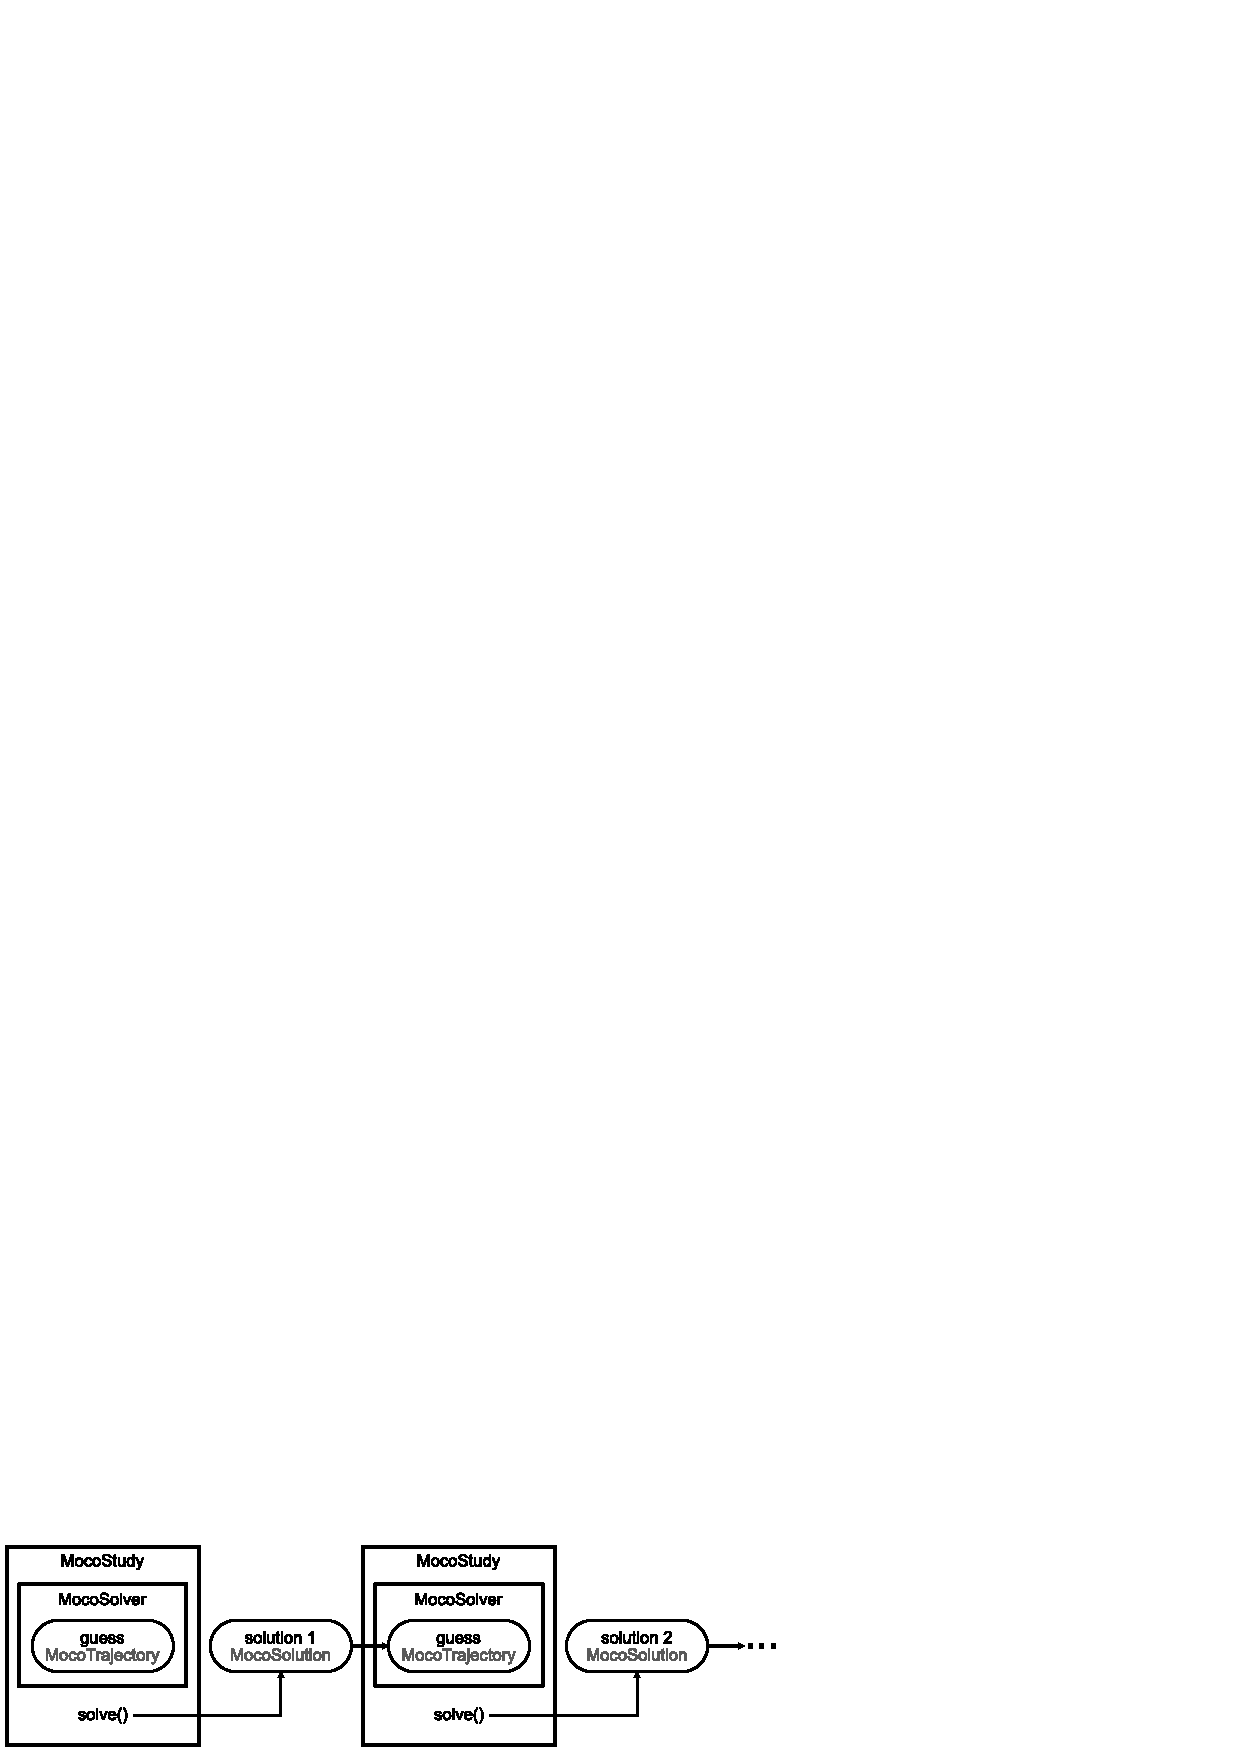
\includegraphics{../figures/MocoSolverDiagram.png}
    \caption{{\bf Using trajectories to solve problems iteratively.}
        Guesses for the optimization are specified using \textit{MocoTrajectory}, which holds the values of states, controls, and parameters at any iteration in the optimization. \textit{MocoSolution} is a subclass of \textit{MocoTrajectory} that holds the solution to a study and includes the success status of the optimization, the final objective value, and the number of solver iterations. Users can use the solution of one problem as the initial guess for a subsequent problem.}
    \label{mocosolverdiagram}
    %\end{adjustwidth}
\end{figure}

After solving a problem, Moco can visualize the solution as an animation, plot the state and control trajectories, or compute quantities from the solution. The ability to save \textit{MocoTrajectories} and \textit{MocoStudies} to files allows users to reproduce each other's results, which is essential for sound science~\cite{Peng:2011}.

\subsection*{Tools for standard problems}

Currently, Moco provides two tools for solving standard problems (Fig~\ref{mocotooldiagram}):
\begin{itemize}
\item \textit{MocoInverse} solves the muscle/actuator redundancy problem, wherein we solve for muscle (or other actuator) controls that achieve a motion that is prescribed exactly (see S1 Appendix) while minimizing effort or other costs.
\item \textit{MocoTrack} solves motion tracking problems, wherein we solve for both a motion and muscle (or other actuator) controls that minimize the error compared to an observed motion in addition to effort or other costs.
\end{itemize}
\textit{MocoTrack} is useful for predicting deviations from motion data (e.g., predicting kinematic adaptations to an exoskeleton), while \textit{MocoInverse} is a faster option when the motion should be enforced exactly (e.g., estimating elastic energy storage for an observed motion). \textit{MocoTrack} can use contact models, while \textit{MocoInverse} can apply measured external forces to the model. For both tools, the only required inputs are an OpenSim model and motion data (coordinate or marker trajectories, and external forces). Internally, the tools build a \textit{MocoStudy} with solver settings that yield fast and reliable convergence on problems we tested.

% Place figure captions after the first paragraph in which they are cited.
\begin{figure}[!h]
    %\begin{adjustwidth}{-2.25in}{0in} % Comment out/remove adjustwidth environment if table fits in text column.
    \centering
    % 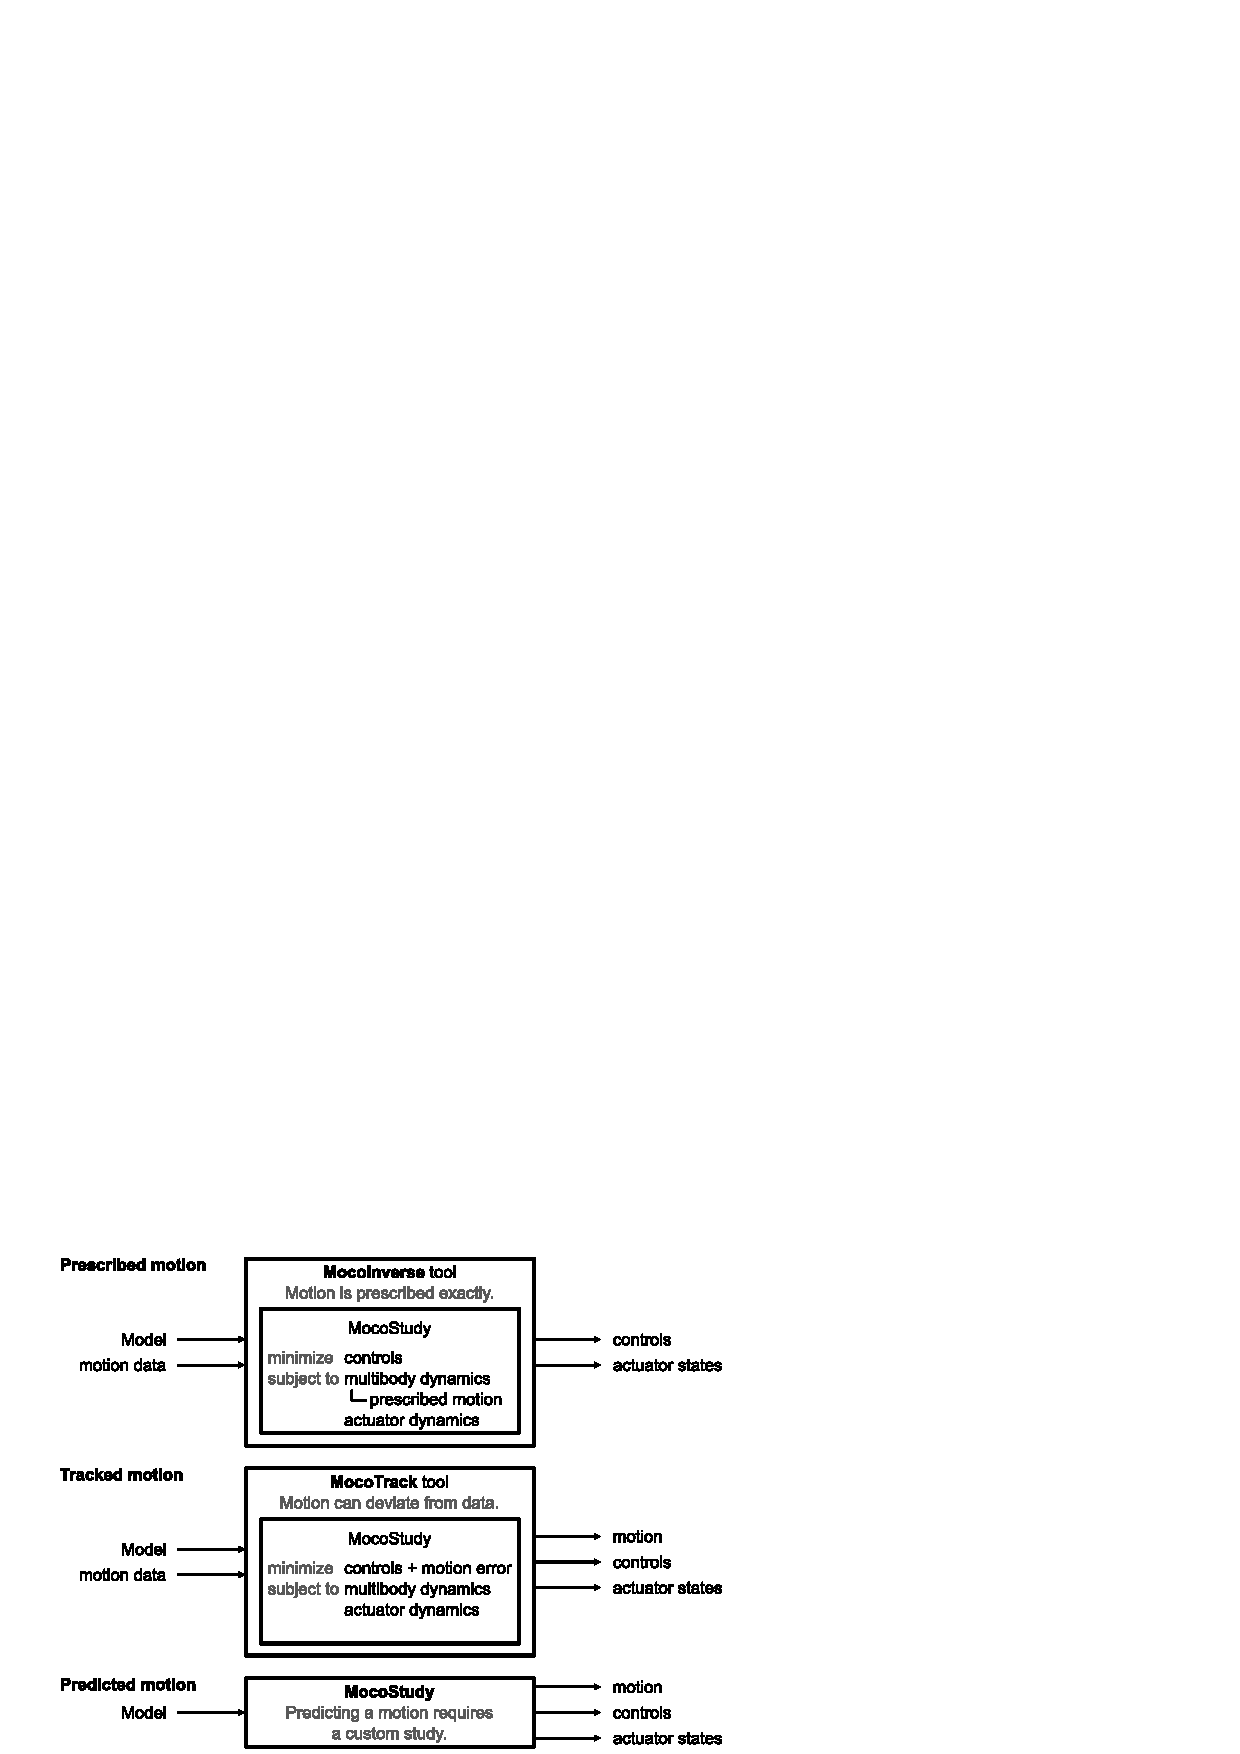
\includegraphics{../figures/MocoToolDiagram.png}
    \caption{{\bf Solving prescribed motion, tracked motion, and predicted motion problems.}
        Moco provides the tools \textit{MocoTrack} and \textit{MocoInverse} for solving standard problems. Both require a \textit{Model} and kinematic data as inputs and produce controls and actuator states as outputs, but these tools solve different optimal control problems. \textit{MocoTrack} produces a new simulated motion, while \textit{MocoInverse} does not permit deviations from the provided kinematic data. Predicting a motion is not easily standardized and requires a custom \textit{MocoStudy}.
    }
    \label{mocotooldiagram}
    %\end{adjustwidth}
\end{figure}

Future versions of Moco may include tools for model calibration, electromyography-driven simulation, and other standard problems. For problems that do not fit into a standard form, such as predicting a motion, \textit{MocoStudy} provides the necessary flexibility.


\subsection*{Verification}

Verifying software is essential~\cite{Hicks:2015bo}; thus, we conducted extensive verification tests. For example, to verify that Moco implements direct collocation correctly we solved the ``linear tangent steering'' optimal control problem~\cite{Bryson:1975}, which has a known solution. Moco's solution matched the known solution with a root-mean-square error of $2.7 \times 10^{-5}$.

We also ensured that a time-stepping forward simulation using controls from a motion prediction produced the same motion as in the prediction. This test used a model consisting of a point mass suspended by three muscles (\textit{DeGrooteFregly2016Muscle}) and under the influence of gravity (Fig~\ref{verification}). For this problem, the muscles had activation dynamics and rigid tendons. We first predicted the state and control trajectories to move the point mass between prescribed initial and final positions, starting and ending at rest (Fig~\ref{verification}, gray band). In this prediction, the cost included both the sum of squared muscle excitations and the final time. Then, we used the predicted controls to perform a time-stepping forward simulation using an OpenSim integrator (Fig~\ref{verification}, blue line). The resulting position trajectory of the point mass matched that from the prediction with a root-mean-square error of 0.0051 m (1.8\% of the distance between the initial and final positions). This gives us confidence that Moco enforces the same multibody and muscle dynamics enforced in a time-stepping forward simulation in OpenSim. For more complex problems, conducting a time-stepping forward simulation using controls from a \textit{MocoSolution} requires a stabilizing feedback controller to counteract numerical errors.

% Place figure captions after the first paragraph in which they are cited.
\begin{figure}[!h]
%    \begin{adjustwidth}{-2.25in}{0in} % Comment out/remove adjustwidth environment if table fits in text column.
        \centering
        % \includegraphics{../figures/suspended_mass.png}
        \caption{{\bf Verification of time-stepping and motion tracking.}
            Left: The trajectory of a point mass suspended by three muscles and moving under the influence of gravity ($g$) was simulated using Moco. Right: The activations of the ``left,'' ``middle,'' and ``right'' muscles are shown for different simulations. The original trajectory (gray band) was predicted by minimizing final time and the sum of squared muscle excitations. The time-stepping forward simulation driven with the predicted controls (blue) produced the motion we originally predicted. Tracking the predicted motion with \textit{MocoTrack} (orange) produced the original activations.
        }
        \label{verification}
%    \end{adjustwidth}
\end{figure}

To gain confidence in motion tracking problems, we ensured that using \textit{MocoTrack} on a synthesized motion with known muscle activity produced the original muscle activity. We used the same suspended point mass model and tracked the previous motion prediction (Fig 6, gray band) while minimizing squared excitations. The muscle activations from \textit{MocoTrack} (Fig 6, orange line) matched those from the prediction with a root-mean-square error that was 0.47\% of the peak predicted activation. For most tracking problems of interest, we do not know the true muscle activity solution; verifying tracking problems using synthesized data gives us confidence in Moco’s estimates of muscle activity.

Moco contains an automated test suite with over 30 files that extends beyond the verification described here. For example, the test suite ensures that users receive error messages for incorrect input, that a \textit{MocoStudy} can be written to and read from an XML file, that kinematic constraints are enforced, and that implicit and explicit differential equations are consistent. We ensure all these tests succeed before accepting changes to the code.

\section*{Results}

\subsection*{Prescribing a walking motion to estimate muscle activity}

Moco can estimate muscle activity in walking, which allows studying muscle coordination in healthy and pathological gait. We used a model with 33 degrees of freedom and 80 lower-limb muscles~\cite{Rajagopal:2016ek} to simulate one gait cycle of walking at a self-selected speed of 1.24 m/s. The scaled model and data are based on the supplementary material of~\cite{Rajagopal:2016ek}. We modeled activation dynamics in all muscles but only modeled tendon compliance in the gastrocnemii and soleus, where a rigid-tendon assumption is less valid~\cite{Groote:2016dq}. We solved for muscle activity using \textit{MocoInverse}, which prescribes kinematics exactly (see ``Tools for standard problems'' for details), and compared the resulting muscle activations to electromyography measurements (Fig~\ref{walking}; black lines and gray shading).

% Place figure captions after the first paragraph in which they are cited.
\begin{figure}[!h]
    % \begin{adjustwidth}{-2.25in}{0in} % Comment out/remove adjustwidth environment if table fits in text column.
    \centering
    % \includegraphics{../figures/motion_prescribed_walking.png}
    \caption{{\bf Estimates of muscle activity during walking.}
        \textit{MocoInverse} produced muscle activations (black) whose timing matched the timing from electromyography measurements (gray). Electromyography for gluteus maximus and iliacus comes from~\cite{Perry:2010}; electromyography for all other muscles comes from~\cite{Rajagopal:2016ek} and was normalized such that its peak matched the peak of the \textit{MocoInverse} activations. Minimizing knee joint loading reduced the activity of the biceps femoris short head, and medial gastrocnemius, which span the knee (blue), and increased the activity of other muscles to compensate.
    }
    \label{walking}
    % \end{adjustwidth}
\end{figure}

\textit{MocoInverse} produced activations that included some of the major features of the electromyography data, such as the timing of peak activity for the semitendinosus, biceps femoris short head, vastus lateralis, medial gastrocnemius, and soleus. Activity for the iliacus was much higher than measured in a separate data set~\cite{Perry:2010} because other hip flexor muscles in the model (which have larger hip adduction moment arms) remained inactive to avoid counteracting the required hip abduction net joint moment. With \textit{MocoInverse}, the difference between required net joint moments and muscle-generated net joint moments (termed ``reserve'' moments) were restricted to be no greater than 2.5 N-m across time and degrees of freedom, which is in accordance with established guidelines (reserve moments are below 5\% of peak net joint moments~\cite{Hicks:2015bo}). \textit{MocoInverse} solved this problem in 2.8 minutes using a 3.6 GHz Intel Core i7 processor with 8 parallel threads; this duration is similar to the amount of time required by the Computed Muscle Control~\cite{Thelen:2003bba} tool in OpenSim for solving prescribed motion problems as reported by Rajagopal and colleagues~\cite{Rajagopal:2016ek}.

To demonstrate Moco's customizability, we added a cost term to \textit{MocoInverse} to minimize knee joint loading. With this additional cost, the average magnitude of the knee joint reaction force decreased from 1.8 to 1.1 body weights. As expected, the activity of muscles crossing the knee joint (vastus lateralis, biceps femoris short head, and medial gastrocnemius) decreased (Fig~\ref{walking}; blue lines). To compensate for the reduced medial gastrocnemius moment at the ankle, soleus activity increased, as seen in a previous simulation study~\cite{DeMers:2014}. Moco solved this problem in 8.2 minutes.

\subsection*{Tracking a walking motion with healthy and weakened muscles}

In addition to producing initial guesses for predictive optimizations, tracking problems (where motion tracking is part of the cost function rather than exactly prescribed) can be useful for studying how changes to a model affect its ability to reproduce a reference motion. Moco provides the \textit{MocoTrack} tool for constructing and solving tracking simulations. With this tool, the cost includes terms for motion tracking and control effort. We explored the effect of weakening different muscle groups in a lower extremity walking model on the model's ability to track healthy walking data. As inputs to \textit{MocoTrack}, we used the same model and walking data as for the \textit{MocoInverse} problem above, with one major addition: the model now included compliant foot-ground contact force elements on both feet~\cite{Falisse:2019b}. We removed the torque actuators serving as ``reserve'' moments, which were only necessary for \textit{MocoInverse}, so that the lower limbs were entirely muscle-driven. We added constraints so the model walked with the same average speed as in the reference data and the feet could not interpenetrate. We assumed mediolateral symmetry and simulated half of a gait cycle.

We first solved the tracking problem using the model's normal (``healthy'') muscle strengths (maximum isometric forces). \textit{MocoTrack} produced ground reaction forces whose timing matched that of the sagittal plane experimental ground reaction forces (Fig~\ref{tracking}, left). Muscle activations for many major lower extremity muscles were qualitatively similar to electromyography data including gluteus maximus, biceps femoris short head, vastus lateralis, medial gastrocnemius, soleus, and tibialis anterior (Fig~\ref{tracking}, activations). Using the same computer as for the \textit{MocoInverse} problems, \textit{MocoTrack} solved this problem in 104 minutes; this duration is shorter than that commonly seen in single-shooting predictions~\cite{Ong:2019}, but is longer than what can be achieved when combining algorithmic differentiation with direct collocation~\cite{Falisse:2019b}.

% Place figure captions after the first paragraph in which they are cited.
\begin{figure}[!h]
    % \begin{adjustwidth}{-2.25in}{0in} % Comment out/remove adjustwidth environment if table fits in text column.
    \centering
    % \includegraphics{../figures/motion_tracking_walking.png}
    \caption{{\bf Tracking 3-D experimental motion data.}
        Left: \textit{MocoTrack} produced sagittal plane ground reaction forces (black) whose timing matched experimentally-measured ground reaction forces (gray). However, the magnitude in the first peak of the vertical ground reaction force was overestimated. Right: Similar to \textit{MocoInverse}, \textit{MocoTrack} produced muscle activations (black) that matched the timing of electromyography measurements (gray). Electromyography for gluteus maximus and iliacus comes from~\cite{Perry:2010}; electromyography for all other muscles come from~\cite{Rajagopal:2016ek} and signals were again normalized such that their peak matched the peak of the \textit{MocoInverse} activations to be consistent with Fig~\ref{walking}.
    }
    \label{tracking}
    % \end{adjustwidth}
\end{figure}

We next weakened the ankle dorsiflexor muscles (tibialis anterior, extensor digitorum longus, and extensor hallucis longus) by reducing max isometric forces by 95\% and solved the tracking problem again. \textit{MocoTrack} produced a ``drop foot'' walking solution, where the model was unable to dorsiflex the ankle in early stance and in swing (Fig~\ref{weakness}, left). We solved the problem again after restoring the dorsiflexor muscle strengths and weakening the hip abductor muscles (gluteus medius, gluteus minimus, and tensor fascia lata) by 90\%. Since major hip abductor forces were nearly reduced to zero (e.g., gluteus medius), the model was unable to produce the hip adduction angle observed in the experimental data and healthy tracking solution, and the adapted gait included a large increase in truck sway (Fig~\ref{weakness}, right). \textit{MocoTrack} solved the weakened dorsiflexor and hip abductor problems in 61 and 55 minutes, respectively.

% Place figure captions after the first paragraph in which they are cited.
\begin{figure}[!h]
    % \begin{adjustwidth}{-2.25in}{0in} % Comment out/remove adjustwidth environment if table fits in text column.
    \centering
    % \includegraphics{../figures/motion_tracking_walking.png}
    \caption{{\bf Effect of weakened dorsiflexors and hip abductors on motion tracking.}
        Left: Weakening the ankle dorsiflexors caused ankle plantarflexion to increase during early stance and swing (orange) compared to the experimental ankle angle (gray) and the healthy tracking solution (black). The tibialis anterior force is normalized by the muscle's healthy max isometric force, $F_\mathrm{iso}$. Right: Weakening the hip abductors resulted in a reduced hip adduction angle (green) during stance compared to the experimental hip adduction angle (gray) and the healthy tracking solution (black). As shown in the skeleton graphic, increased trunk sway was observed (green) compared to the healthy tracking solution (white). The force in the gluteus medius, a primary hip abductor, was nearly reduced to zero across the gait cycle.
    }
    \label{weakness}
    % \end{adjustwidth}
\end{figure}

\subsection*{Predicting and assisting a squat-to-stand motion}

To show that Moco can predict motions and optimize parameters of a model, we predicted a squat-to-stand motion that minimized a combination of effort, expressed as the sum of squared excitations, and the duration of the motion. The initial pose was prescribed to be squatting~\cite{Fregly:2015}, and the final pose was prescribed to be upright standing. No motion was tracked. The model contained a torso and a single leg with 9 muscles obeying activation dynamics and compliant tendon dynamics; muscle strengths were based on those from a previous study~\cite{Ong:2019}. We used Moco's default initial guess, in which each variable's value is the midpoint of the variable's bounds. The predicted motion and muscle activations are shown in Fig~\ref{squattostand} (black lines). As expected, extensor muscles such as the gluteus maximus, hamstrings, and vasti exhibited the greatest activity.

% Place figure captions after the first paragraph in which they are cited.
\begin{figure}[!h]
    % \begin{adjustwidth}{-2.25in}{0in} % Comment out/remove adjustwidth environment if table fits in text column.
        \centering
        % \includegraphics{../figures/squat_to_stand.png}
        \caption{{\bf Predicting and assisting a squat-to-stand motion.}
            Left: We predicted a squat-to-stand motion with prescribed initial and final poses that minimized the sum of squared muscle excitations and final time, then added a torsional spring to the knee and solved for the optimal spring stiffness $k$. Right: The activations of key muscles throughout the motion without (black) and with (blue) the assistive spring show that the spring allowed gluteus maximus and vasti activity to decrease substantially.
        }
        \label{squattostand}
    % \end{adjustwidth}
\end{figure}

Next, we added a torsional spring to the knee and solved for the optimal motion, muscle activations, and spring stiffness. The spring was in equilibrium when the knee was extended, as illustrated in Fig~\ref{squattostand}. We used the same cost as in the unassisted case; no motion was tracked. With the assistive device, the motion was achieved with lower muscle activity. The optimal spring stiffness was 90 N-m/rad.

Both predictions converged in 3 minutes. Moco's ability to rapidly predict motions and optimize device parameters makes it a valuable tool for designing assistive devices.

The duration of the various optimizations presented in this section are summarized in Table 1.

\begin{table}[!ht]
    \begin{adjustwidth}{-2.25in}{0in} % Comment out/remove adjustwidth environment if table fits in text column.
        \centering
        \caption{
            {\bf Duration of optimization problems.}}
        \begin{tabular}{|l|l|}
            \hline
            {\bf problem} & {\bf duration (minutes)} \\ \thickhline
            MocoInverse, gait (Fig 7, black) & 2.8 \\ \hline
            MocoInverse, gait, minimizing knee load (Fig 7, blue) & 8.2 \\ \hline
            MocoTrack, gait, healthy (Fig 8) & 104 \\ \hline
            MocoTrack, gait, weak dorsiflexors (Fig 9, orange) & 61 \\ \hline
            MocoTrack, gait, weak hip abductors (Fig 9, green) & 55 \\ \hline
            Predictive MocoStudy, squat-to-stand, unassisted (Fig 10, black) & 3 \\ \hline
            Predictive MocoStudy, squat-to-stand, assisted (Fig 10, blue) & 3 \\ \hline
        \end{tabular}
        \begin{flushleft}
            Durations were obtained with a
            3.6 GHz Intel Core i7 processor with 8 parallel threads.
        \end{flushleft}
        \label{tab:durations}
    \end{adjustwidth}
\end{table}

\section*{Availability and future directions}

OpenSim Moco is free to download for Windows and Mac on Moco's website (\\https://opensim.stanford.edu/moco) and SimTK (https://simtk.org/projects/opensim-moco). The source code is available on GitHub (https://github.com/opensim-org/opensim-moco). Moco's source code is licensed under the permissive Apache License 2.0, though some dependencies have more restrictive licenses (e.g., CasADi~\cite{Andersson:2019} is available under the GNU Lesser General Public License).

The documentation for Moco is extensive. The User Guide that explains how to use Moco and provides tips for posing a problem, the Theory Guide explains how Moco implements direct collocation, the Application Programming Interface (API) Reference describes the classes and functions in the library, and the Developer Guide explains our software design. We provide a two-page ``cheat sheet'' that demonstrates common commands. Moco contains examples in MATLAB, Python, and C++ that range from predicting the optimal trajectory for a double pendulum to predicting 2-D muscle-driven walking (which solves in 30 minutes). The code that generated the results for this paper are available at https://github.com/stanfordnmbl/mocopaper.

Going forward, we will focus on applying Moco to high-impact scientific questions in biomechanics. Moco brings biomechanists closer than ever before to predicting outcomes of orthopedic surgeries and rehabilitation strategies such as tendon surgeries and muscle strength training. Predictions of movement typically employ generic models because large-scale subject-specific simulations are difficult to build. Moco permits researchers to easily build and share subject-specific studies that could discern which individuals may benefit from an intervention. Using Moco with inertial measurement units~\cite{Dorschky:2019} or video data will allow researchers to analyze and predict muscle behavior for movements based on observations outside of the laboratory.

We believe Moco's community will be its strongest asset. We have already begun building this community by hosting workshops that have put Moco in the hands of over 100 researchers. We will grow this community through additional workshops at conferences, at Stanford University, and online, and by helping others to contribute documentation, examples, teaching materials, and code.

We designed Moco to be easy to use, customizable, and extensible. We verified the software and applied it to multiple musculoskeletal problems. Moco handles models with kinematic constraints, muscle activation dynamics, compliant tendons, and compliant contact, and can minimize a combination of complex costs such as marker tracking and joint reaction loads. Given this foundation, we expect Moco to accelerate research by reducing the time spent wrestling with simulation tools and enabling our field to tackle more ambitious problems.

\section*{Acknowledgments}

We thank Ajay Seth, Michael Sherman, Friedl de Groote, Michael Posa, Joris Gillis, and Joel Andersson for discussing methodology and implementation; Bradley Humphreys, Carmichael Ong, Noah Gordon, and Jennifer Yong for contributing code; Andrew Baines, Mohammad Shourijeh, and Prasanna Sritharan for testing the software; and Ayman Habib for reviewing the manuscript.

\section*{Supporting information}

\paragraph*{S1 Appendix.}
\label{S1_Appendix}
{\bf Mathematical details.} This appendix describes in detail how Moco solves optimal control problems with direct collocation.

\paragraph*{S2 Source code.}
\label{S2_SourceCode}
{\bf Source code for OpenSim Moco.} This file contains the source code for version 0.4.0 of OpenSim Moco, which was used to generate the results.

\paragraph*{S3 Documentation.}
\label{S3_Documentatino}
{\bf Documentation for OpenSim Moco.} This file contains documentation (in HTML) for OpenSim Moco.

\nolinenumbers

% Either type in your references using
% \begin{thebibliography}{}
% \bibitem{}
% Text
% \end{thebibliography}
%
% or
%
% Compile your BiBTeX database using our plos2015.bst
% style file and paste the contents of your .bbl file
% here. See http://journals.plos.org/plosone/s/latex for
% step-by-step instructions.
%

\bibliography{MocoPaper.bib}

%\begin{thebibliography}{10}
%
%\bibitem{bib1}
%Conant GC, Wolfe KH.
%\newblock {{T}urning a hobby into a job: how duplicated genes find new
%  functions}.
%\newblock Nat Rev Genet. 2008 Dec;9(12):938--950.
%
%\bibitem{bib2}
%Ohno S.
%\newblock Evolution by gene duplication.
%\newblock London: George Alien \& Unwin Ltd. Berlin, Heidelberg and New York:
%  Springer-Verlag.; 1970.
%
%\bibitem{bib3}
%Magwire MM, Bayer F, Webster CL, Cao C, Jiggins FM.
%\newblock {{S}uccessive increases in the resistance of {D}rosophila to viral
%  infection through a transposon insertion followed by a {D}uplication}.
%\newblock PLoS Genet. 2011 Oct;7(10):e1002337.
%
%\end{thebibliography}



\end{document}


